% ============================================================
%  FasiTech -- Proposta para Prêmio de Inovação UFPA 2026
%  Anexo II – Roteiro do relato da ação inovadora
%  Documento sem identificação dos proponentes (julgamento cego)
% ============================================================
\documentclass[12pt,a4paper]{article}

% ------ Codificação e língua ------
\usepackage[utf8]{inputenc}
\usepackage[T1]{fontenc}
\usepackage[brazil]{babel}

% ------ Layout de página ------
\usepackage[top=2.5cm, bottom=2.5cm, left=3cm, right=2.5cm]{geometry}

% ------ Tipografia ------
\usepackage{microtype}
\usepackage{lmodern}
\usepackage{setspace}
\setstretch{1.13}

% ------ Gráficos e cores ------
\usepackage{graphicx}
\usepackage{float}
\usepackage{caption}
\graphicspath{{Img/}}
\usepackage{xcolor}
\definecolor{ufpablue}{RGB}{0,55,115}
\definecolor{ufpared}{RGB}{175,28,28}
\definecolor{darkgreen}{RGB}{0,110,45}
\definecolor{accentor}{RGB}{210,100,0}
\definecolor{lightblue}{RGB}{220,235,255}
\definecolor{lightgreen}{RGB}{215,245,225}
\definecolor{lightyellow}{RGB}{255,250,215}

% ------ TikZ ------
\usepackage{tikz}
\usetikzlibrary{shapes.geometric, arrows.meta, positioning, fit,
                backgrounds, calc, matrix, shadows}

% ------ FontAwesome 5 ------
\usepackage{fontawesome5}

% ------ Tabelas ------
\usepackage{booktabs}
\usepackage{tabularx}
\usepackage{multirow}
\usepackage{array}
\newcolumntype{L}[1]{>{\raggedright\arraybackslash}p{#1}}
\newcolumntype{C}[1]{>{\centering\arraybackslash}p{#1}}

% ------ Listas ------
\usepackage{enumitem}
\setlist[itemize]{itemsep=2pt, topsep=4pt}
\setlist[enumerate]{itemsep=2pt, topsep=4pt}

% ------ Caixas coloridas ------
\usepackage{tcolorbox}
\tcbuselibrary{skins, breakable}
\tcbset{
  metricbox/.style={
    enhanced, colback=lightblue, colframe=ufpablue!65,
    arc=5pt, boxrule=0.8pt, left=6pt, right=6pt, top=4pt, bottom=4pt,
    fonttitle=\bfseries\small
  },
  successbox/.style={
    enhanced, colback=lightgreen, colframe=darkgreen!60,
    arc=5pt, boxrule=0.8pt, left=6pt, right=6pt, top=4pt, bottom=4pt
  },
  warnbox/.style={
    enhanced, colback=lightyellow, colframe=accentor!70,
    arc=5pt, boxrule=0.8pt, left=6pt, right=6pt, top=4pt, bottom=4pt
  }
}

% ------ Links ------
\usepackage{hyperref}
\hypersetup{colorlinks=true, linkcolor=ufpablue, urlcolor=ufpablue}

% ------ Títulos de seção ------
\usepackage{titlesec}
\titleformat{\section}{\normalsize\bfseries\color{ufpablue}}
  {\thesection}{0.5em}{}[\vspace{-2pt}\color{ufpablue!50}\hrule\vspace{2pt}]
\titlespacing{\section}{0pt}{10pt}{4pt}
\setcounter{secnumdepth}{0}

% ------ Cabeçalho/rodapé ------
\usepackage{fancyhdr}
\pagestyle{fancy}
\fancyhf{}
\renewcommand{\headrulewidth}{0.4pt}
\fancyhead[L]{\footnotesize\color{gray} Prêmio de Inovação em Processos Organizacionais da UFPA -- Edição 2026}
\fancyhead[R]{\footnotesize\color{gray} \thepage}
\fancyfoot{}

% ============================================================
\begin{document}
% ============================================================

% ---- Título ----
\begin{center}
  {\large\bfseries\color{ufpablue}
    FasiTech: Plataforma Digital Integrada para Gestão Acadêmica\\[3pt]
    em Campus Multicampi no Interior da Amazônia}\\[6pt]
  {\small Data de implementação: 01/10/2025 \quad|\quad
   Unidade: [identificação omitida para julgamento cego]}
\end{center}

% \vspace{4pt}
% \begin{tcolorbox}[metricbox]
%   \textbf{\faBook\;Objetivos do PDI 2016-2025 impactados:}
%   (1)~\textit{Melhorar e fortalecer a governança dos processos internos};
%   (2)~\textit{Expandir e aperfeiçoar a gestão institucional na perspectiva multicampi};
%   (3)~\textit{Assegurar a disponibilidade de sistemas essenciais de Tecnologia da Informação};
%   (4)~\textit{Aprimorar a comunicação institucional}.
% \end{tcolorbox}
% \vspace{6pt}

% ============================================================
\section{1\;–\;Qual era a situação-problema a ser enfrentada?}
% ============================================================

A unidade acadêmica, localizada em um campus no interior da Amazônia, atende
estudantes distribuídos em três polos geograficamente dispersos: polo sede, polo remoto A
e polo remoto B. Essa configuração \textit{multicampi} impunha desafios que o modelo de
gestão vigente não conseguia superar:

\begin{itemize}[label={\color{ufpared}\faExclamationCircle}]
  \item \textbf{Processos integralmente em papel:} ACC, TCC, Estágio, Plano de Ensino e
    Requerimento de Banca exigiam deslocamento físico do estudante até a secretaria.

  \item \textbf{Deslocamento obrigatório em contexto de alta vulnerabilidade:} Levantamento
    socioeconômico revelou que \textbf{75\% dos estudantes se deslocam a pé ou de bicicleta};
    os dois polos mais distantes da sede concentram em torno 30\%
    dos estudantes e ficam a horas de viagem do polo sede.

  \item \textbf{Cálculo manual de carga horária de ACC:} A secretaria somava manualmente
    as cargas horárias de cada certificado físico, processo suscetível a erros e
    representando gargalo operacional significativo.

  \item \textbf{Ausência de dados socioeconômicos estruturados:} A coordenação não dispunha
    de perfil sistematizado dos estudantes, inviabilizando políticas de permanência e
    assistência estudantil baseadas em evidências.

  \item \textbf{Comunicação reativa e não rastreável:} Prazos acadêmicos críticos eram
    comunicados via grupos de mensagens, sem registro, sem padronização e sem confirmação de
    recebimento.

  \item \textbf{Gestão sem indicadores de satisfação:} Não havia mecanismo formal para
    medir a percepção dos estudantes sobre a gestão acadêmica.
\end{itemize}

Esse cenário contrariava o objetivo estratégico do PDI/UFPA de \textit{``aperfeiçoar
processos e procedimentos que impulsionem a fluidez na gestão''} e de \textit{``consolidar
a atuação institucional em sistema multicampi''}. Para um público em que \textbf{78,4\%
vivem com renda familiar de até 1 salário mínimo}, cada deslocamento ao campus tem custo
real e o sistema pré-existente transferia esse custo ao estudante.

% ============================================================
\section{2\;–\;Qual foi a ação de inovação em processos implementada?}
% ============================================================

O \textbf{FasiTech} é uma plataforma digital integrada de gestão acadêmica e administrativa
desenvolvida para a subunidade acadêmica. Reúne em um único ambiente web os principais processos de
tramitação entre estudantes, docentes e secretaria, organizados em dez módulos funcionais:

\begin{center}
\begin{tikzpicture}[
  box/.style={rectangle, rounded corners=4pt, minimum width=3.0cm, minimum height=0.9cm,
              text width=2.85cm, align=center, font=\footnotesize\bfseries, drop shadow},
  core/.style={box, fill=ufpablue, text=white, minimum width=3.4cm},
  mstud/.style={box, fill=ufpablue!18, draw=ufpablue!55, text=ufpablue!85!black},
  mdoc/.style={box, fill=darkgreen!18, draw=darkgreen!55, text=darkgreen!80!black},
  mai/.style={box, fill=accentor!18, draw=accentor!55, text=accentor!80!black},
  arr/.style={-{Stealth[length=4pt]}, thick, color=gray!60}
]
% Core
\node[core] (core) at (0,0) {\faDatabase\; Portal FasiTech\\[1pt]{\tiny Backend + Banco de Dados}};

% Módulos do aluno (esquerda e cima)
\node[mstud] (acc)  at (-3.6, 2.2)  {\faFilePdf\; ACC};
\node[mstud] (tcc)  at (0,    2.2)  {\faGraduationCap\; TCC};
\node[mstud] (est)  at ( 3.6, 2.2)  {\faBriefcase\; Estágio};
\node[mstud] (soc)  at (-3.6,-2.2)  {\faUsers\; Perfil Social};
\node[mstud] (req)  at (0,   -2.2)  {\faFileSignature\; Req.\ Banca};
\node[mstud] (aval) at ( 3.6,-2.2)  {\faChartBar\; Aval.\ Gestão};

% Módulos do docente / secretaria (direita)
\node[mdoc]  (proj) at ( 4.8, 0.7)  {\faFolderOpen\; Projetos};
\node[mdoc]  (plan) at ( 4.8,-0.7)  {\faChalkboardTeacher\; Plano Ensino};

% Módulos de IA/automação (esquerda)
\node[mai]   (dir)  at (-4.8, 0.7)  {\faRobot\; Diretor Virtual\\[-1pt]{\tiny IA + RAG}};
\node[mai]   (not)  at (-4.8,-0.7)  {\faCogs\; Lançamento\\[-1pt]{\tiny de Conceitos}};

% Alertas (topo direito do core)
\node[mstud] (ale)  at ( 8.6, 0)    {\faBell\; Alertas\\[-1pt]Acadêmicos};

% Arrows
\foreach \n in {acc,tcc,est,soc,req,aval,proj,plan,dir,not,ale}
  \draw[arr] (\n) -- (core);

\end{tikzpicture}
\end{center}

\begin{center}
  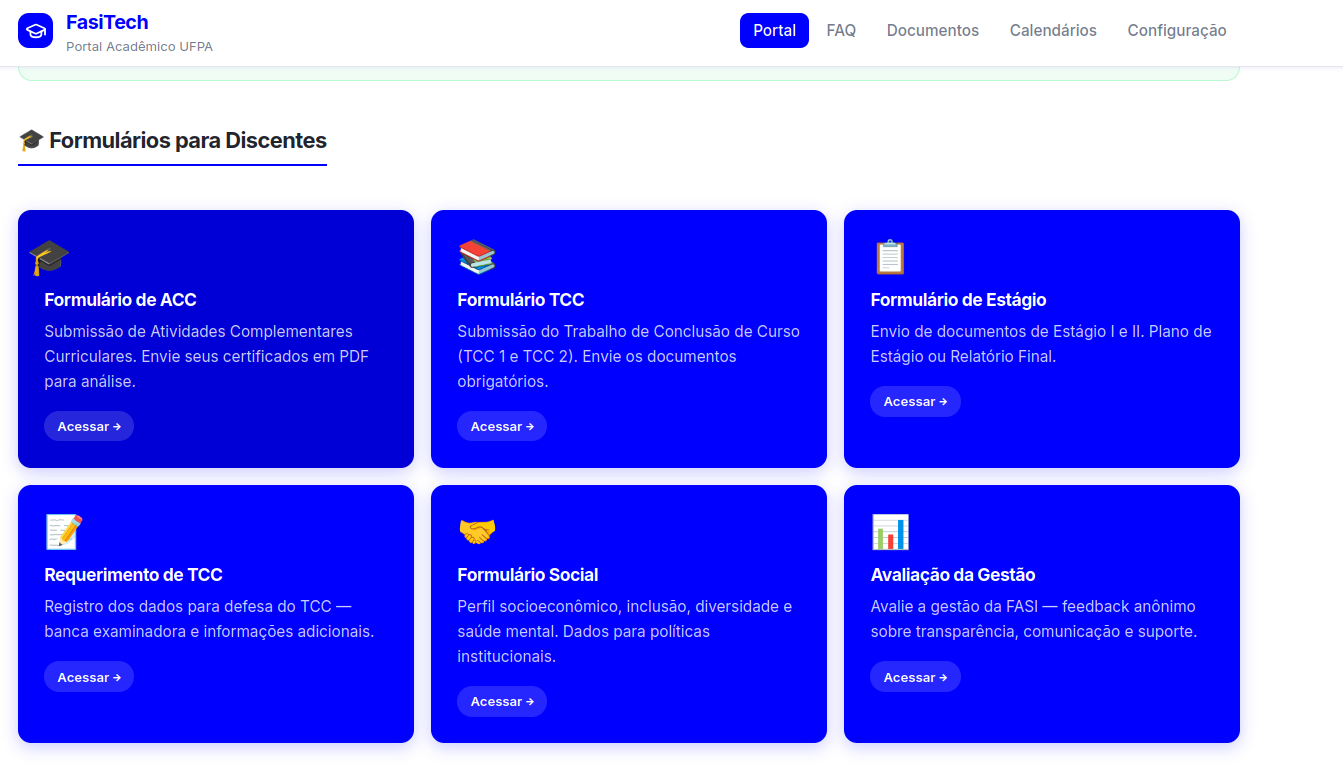
\includegraphics[width=0.49\linewidth]{PagePrincipal_View1}\hfill%
  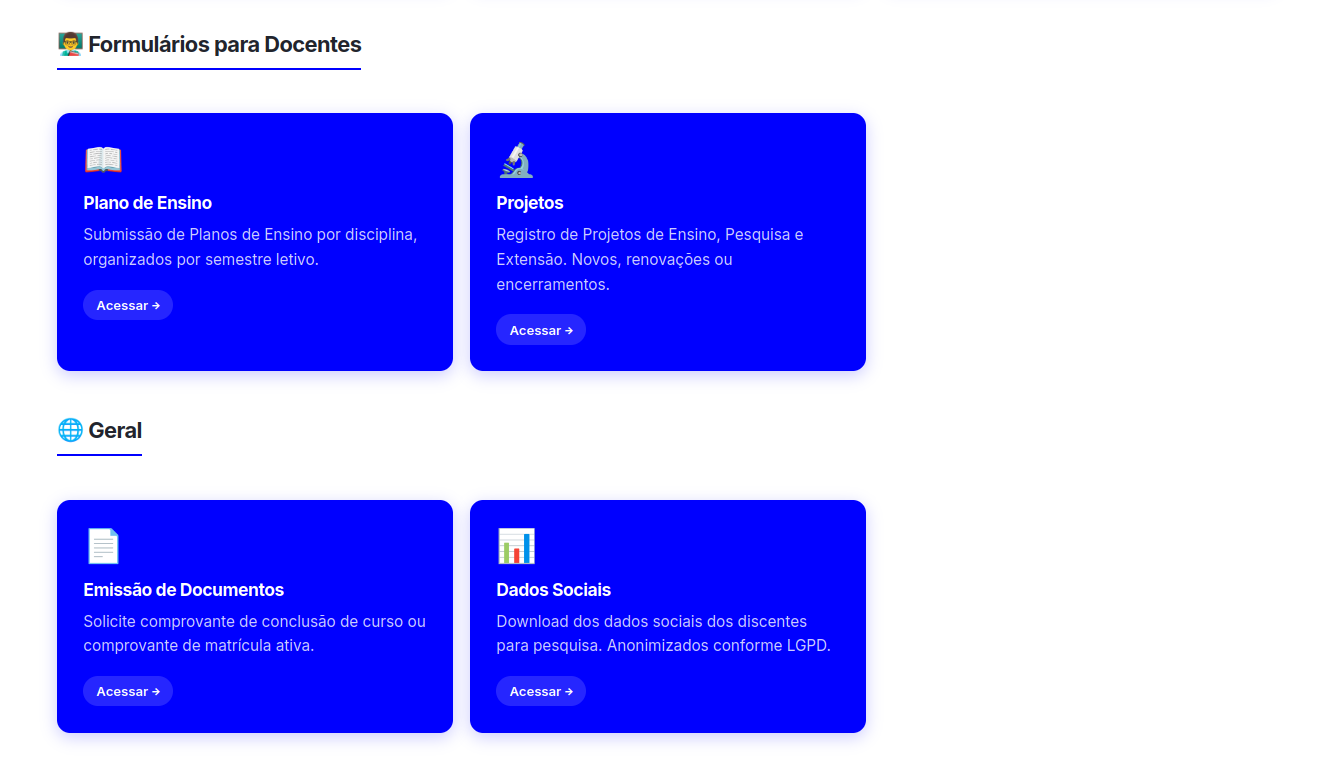
\includegraphics[width=0.49\linewidth]{PagePrincipal_View2}\\[2pt]
  {\scriptsize\textit{Portal FasiTech: formulários para discentes (esq.) e para docentes / área geral (dir.)}}
\end{center}

\vspace{4pt}
Dois módulos utilizam \textbf{automação inteligente} que diferencia o sistema de soluções
convencionais:

\begin{itemize}[label={\color{accentor}\faRobot}]
  \item \textbf{Módulo ACC com IA:} Os certificados são enviados como arquivos PDF.
    Um modelo de Inteligência Artificial extrai automaticamente as cargas horárias de cada
    documento, elimina o cálculo manual e retorna ao estudante um resumo validado. Processo que antes consumia horas da secretaria.

  \item \textbf{Diretor Virtual (IA/RAG):} Assistente conversacional que utiliza a
    técnica de \textit{Retrieval-Augmented Generation} (RAG), combinando busca em
    documentos institucionais (PPC, regulamentos) com geração de respostas em linguagem
    natural. Disponível 24 horas, em todos os polos, sem intervenção humana.
\end{itemize}

\begin{center}
  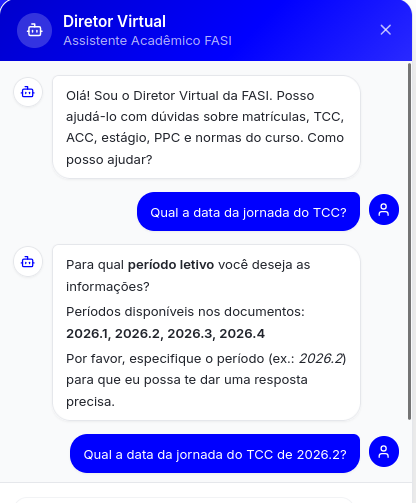
\includegraphics[width=0.30\linewidth]{DiretorVirtual_view1}\hspace{0.06\linewidth}%
  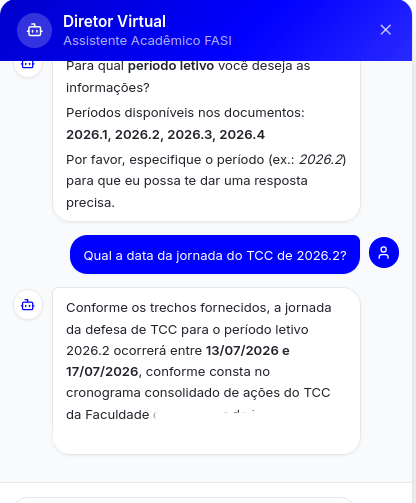
\includegraphics[width=0.30\linewidth]{DiretorVirtual_view2}\\[2pt]
  {\scriptsize\textit{Diretor Virtual: detecção automática de ambiguidade temporal e resposta
  precisa com data do período letivo consultado.}}
\end{center}

\vspace{4pt}
\begin{tcolorbox}[warnbox,
  title={\faCogs\; Pipeline RPA para Projetos de Ensino, Pesquisa e Extensão},
  fonttitle=\bfseries\small\color{accentor!80!black}]

\noindent Ao submeter um projeto, o FasiTech executa automaticamente um
\textbf{pipeline de automação documental de ponta a ponta}, sem intervenção manual
da secretaria:

\vspace{4pt}
\noindent\resizebox{\linewidth}{!}{%
\begin{tikzpicture}[
  node distance=0.30cm,
  flownode/.style={rectangle, rounded corners=4pt, fill=accentor!14, draw=accentor!55,
               minimum width=2.6cm, minimum height=1.1cm, align=center, font=\small\bfseries},
  arr/.style={-{Stealth[length=5pt]}, thick, color=accentor!65}
]
\node[flownode] (form)  {Submissão\\via Portal Web};
\node[flownode, right=of form]  (drive) {Artefatos no\\Google Drive\\{\tiny (por edital/docente)}};
\node[flownode, right=of drive] (pdf)   {Parecer PDF\\gerado\\{\tiny (automático)}};
\node[flownode, right=of pdf]   (email) {E-mail aos\\Pareceristas\\{\tiny (link + PDF)}};
\node[flownode, right=of email] (bd)    {Registro\\no Banco\\{\tiny (auditável)}};
\draw[arr] (form.east)  -- (drive.west);
\draw[arr] (drive.east) -- (pdf.west);
\draw[arr] (pdf.east)   -- (email.west);
\draw[arr] (email.east) -- (bd.west);
\end{tikzpicture}}

\vspace{5pt}
\begin{itemize}[itemsep=1pt, topsep=0pt, leftmargin=1.2em]
  \item \textbf{Armazenamento estruturado no Google Drive:} pasta hierárquica por edital
    e docente, acervo disponível imediatamente para inspeção do MEC e auditorias internas,
    sem busca manual em e-mails ou drives pessoais.
  \item \textbf{Geração automática do parecer:} PDF com identificação do projeto,
    pareceristas designados e campo de assinatura com nenhuma digitação pela secretaria.
  \item \textbf{Notificação instantânea:} pareceristas recebem, no mesmo instante da
    submissão, link para os artefatos no Drive e o PDF do parecer para leitura e assinatura.
\end{itemize}
\end{tcolorbox}

% ============================================================
\section{3\;–\;Quais são os objetivos da ação?}
% ============================================================

\begin{enumerate}[label={\textbf{\arabic*.}}, leftmargin=*, itemsep=3pt]
  \item Digitalizar \textbf{100\% dos trâmites acadêmicos formais}, eliminando dependência
    de processos em papel e de deslocamento presencial para envio de documentos.
  \item Automatizar tarefas de alto volume e baixo valor agregado (cálculo de horas ACC,
    consolidação de conceitos), liberando a secretaria para atividades estratégicas.
  \item Gerar \textbf{perfil socioeconômico estruturado e longitudinal} dos estudantes,
    provendo base de dados para políticas de assistência e inclusão.
  \item Institucionalizar \textbf{alertas acadêmicos automáticos e rastreáveis},
    substituindo comunicações informais por notificações documentadas.
  \item Criar \textbf{mecanismo contínuo de avaliação da gestão}, com dimensões
    quantitativas e qualitativas, ciclo semestral e transparência dos resultados.
  \item Produzir \textbf{indicadores de uso e impacto em tempo real} para apoiar a
    tomada de decisão da coordenação, em alinhamento com o PDI da UFPA.
  \item Ampliar o acesso ao conhecimento institucional via Diretor Virtual, atendendo
    dúvidas sobre o PPC e processos a qualquer horário, em todos os polos.
\end{enumerate}

% ============================================================
\section{4\;–\;Qual é o público-alvo da ação?}
% ============================================================

\noindent\textbf{Público direto:} aproximadamente 200 estudantes ativos nos três polos
(polo sede, polo remoto A e polo remoto B), o corpo docente e a equipe técnico-administrativa
da subunidade.

\noindent\textbf{Público indireto:} coordenação da faculdade, famílias dos estudantes,
demais campi da UFPA (como potencial de replicação) e a gestão institucional da UFPA,
que se beneficia de indicadores estruturados de uma subunidade multicampi no interior.

\medskip
O perfil socioeconômico levantado pelo próprio FasiTech (n=148) revela um público de
\textbf{alta vulnerabilidade}, para quem a digitalização é condição de equidade:

\begin{center}
\renewcommand{\arraystretch}{1.15}
\begin{tabular}{L{7.8cm} r}
\toprule
\textbf{Indicador} & \textbf{Percentual} \\
\midrule
Renda familiar $\leq$ 1 salário mínimo      & 78,4\% \\
Desloca-se a pé ou de bicicleta             & 75,0\% \\
Não trabalha (dependência de bolsas)        & 70,9\% \\
Autodeclara-se pardo ou preto               & 73,0\% \\
Saúde mental regular/ruim/muito ruim        & 42,6\% \\
Sem acesso estável à internet               & 14,2\% \\
Sem computador próprio                      & 25,0\% \\
\bottomrule
\end{tabular}
\end{center}

% ============================================================
\section{5\;–\;Quais foram as principais etapas da implementação da ação?}
% ============================================================

\begin{center}
\begin{tikzpicture}[
  ph/.style={rectangle,scale=0.8, rounded corners=4pt, text width=2.6cm, minimum height=1.7cm,
             align=center, font=\footnotesize, drop shadow},
  arr/.style={-{Stealth[length=5pt]}, thick, color=ufpablue!60}
]
\node[ph, fill=ufpablue!15, draw=ufpablue!40] (p1) at (0,0)
  {\textbf{Fase 1}\\2020--2024\\{\tiny Diagnóstico e\\mapeamento de\\processos}};
\node[ph, fill=ufpablue!28, draw=ufpablue!55] (p2) at (3.0,0)
  {\textbf{Fase 2}\\Jan--Set/2025\\{\tiny Desenvolvimento\\dos módulos\\centrais}};
\node[ph, fill=ufpablue!50, draw=ufpablue!70, text=white] (p3) at (6.0,0)
  {\textbf{Fase 3}\\Out/2025\\{\tiny Go-live em\\produção:\\66 envios}};
\node[ph, fill=ufpablue!70, draw=ufpablue!85, text=white] (p4) at (9.0,0)
  {\textbf{Fase 4}\\Nov/25--Fev/26\\{\tiny IA + RAG +\\Alertas;\\173 envios/mar}};
\node[ph, fill=ufpablue!90, draw=ufpablue, text=white] (p5) at (12.0,0)
  {\textbf{Fase 5}\\Mar--Jun/2026\\{\tiny Novos módulos;\\extração de\\indicadores}};

\draw[arr] (p1.east) -- (p2.west);
\draw[arr] (p2.east) -- (p3.west);
\draw[arr] (p3.east) -- (p4.west);
\draw[arr] (p4.east) -- (p5.west);
\end{tikzpicture}
\end{center}

\textbf{Fase 1 -- Diagnóstico (2020--2024):} Mapeamento dos processos manuais vigentes,
identificação dos gargalos de maior impacto (cálculo ACC, tramitação em papel, dispersão
geográfica) e migração de dados históricos.

\textbf{Fase 2 -- Desenvolvimento dos módulos centrais (jan--set/2025):} Construção dos
módulos de ACC, TCC, Estágio, Projetos, Plano de Ensino e Perfil Socioeconômico.
Arquitetura baseada em servidor web com banco de dados relacional e interface acessível
por qualquer navegador ou smartphone.

\textbf{Fase 3 -- Lançamento em produção (out/2025):} Implantação com usuários reais.
Primeiro mês: \textbf{66 submissões} $\rightarrow$ evidência imediata de adoção espontânea.
Módulo de alertas acadêmicos ativado.

\textbf{Fase 4 -- Integração de IA e consolidação (nov/2025--fev/2026):} Integração
do processamento de certificados ACC com modelo de IA; desenvolvimento do Diretor
Virtual com RAG; evolução dos módulos de lançamento de conceitos. Março de 2026
registrou \textbf{173 submissões} $\rightarrow$ pico absoluto, coincidente com período de prazos
críticos do calendário acadêmico.

\textbf{Fase 5 -- Expansão e métricas (mar--jun/2026):} Implantação da Avaliação de
Gestão e do Requerimento de Banca. Extração estruturada de indicadores de impacto.
Consolidação de \textbf{468 registros em 10 tabelas transacionais}.

% ============================================================
\section{6\;–\;Por que a ação é inovadora?}
% ============================================================

\begin{tcolorbox}[successbox, title={\faStar\; Dimensões de Inovação do FasiTech},
  fonttitle=\bfseries\small\color{darkgreen!80!black}]

\begin{enumerate}[label={\color{darkgreen}\textbf{\arabic*.}}, itemsep=5pt]
  \item \textbf{Primeira plataforma integrada da subunidade:} Antes do FasiTech, não existia
    qualquer sistema digital unificado para tramitação acadêmica na subunidade. A inovação não
    é incremental, é a \textit{substituição completa} de um modelo papel-dependente por
    um fluxo 100\% digital, cobrindo simultaneamente dez tipos de processo.

  \item \textbf{IA aplicada a burocracia acadêmica:} O uso de Inteligência Artificial para
    leitura e extração de dados de certificados PDF (módulo ACC) é aplicação concreta de
    tecnologia a uma tarefa antes puramente manual. O modelo interpreta documentos
    heterogêneos e calcula automaticamente a carga horária válida por categoria
    curricular com resultado auditável.

  \item \textbf{Assistente Virtual com RAG:} O Diretor Virtual combina busca semântica
    em documentos institucionais com geração de respostas em linguagem natural (RAG),
    democratizando o acesso a informações do PPC e regulamentos em todos os polos,
    a qualquer hora sem depender da disponibilidade da secretaria.

  \item \textbf{Produção inédita de dados socioeconômicos longitudinais:} Pela primeira
    vez a unidade dispõe de 148 perfis estruturados com mais de 20 variáveis por aluno,
    constituindo base de dados original para formulação de políticas de permanência.

  \item \textbf{Custo marginal zero para a instituição:} Desenvolvido com ferramentas de
    código aberto e APIs em camadas gratuitas, sem aquisição de licenças ou contratação
    de serviços externos, demonstrando que inovação pública efetiva não depende de
    novos recursos, mas de competência organizacional e orientação pelo bem público.
\end{enumerate}
\end{tcolorbox}

% ============================================================
\section{7\;–\;Quais foram os principais resultados obtidos pela ação?}
% ============================================================

\subsection*{7.1\;Indicadores quantitativos (outubro/2025 – junho/2026)}

\begin{center}
\renewcommand{\arraystretch}{1.2}
\begin{tabular}{L{8.5cm} r C{2.0cm}}
\toprule
\textbf{Indicador} & \textbf{Resultado} & \textbf{Status} \\
\midrule
Trâmites acadêmicos 100\% digitalizados      & \textbf{222 processos} & \textcolor{darkgreen}{\faCheckCircle} \\
Polos atendidos simultaneamente              & \textbf{3 polos}       & \textcolor{darkgreen}{\faCheckCircle} \\
Pico de adoção mensal (março/2026)           & \textbf{173 envios}    & \textcolor{darkgreen}{\faCheckCircle} \\
Dois polos mais distantes da sede     & \textbf{75,7\% dos envios} & \textcolor{darkgreen}{\faCheckCircle} \\
Alertas acadêmicos disparados no prazo       & \textbf{6/6 (100\%)}   & \textcolor{darkgreen}{\faCheckCircle} \\
Certificados ACC processados por IA          & \textbf{53 PDFs}       & \textcolor{darkgreen}{\faCheckCircle} \\
Taxa de consolidação de conceitos            & \textbf{87,3\%}        & \textcolor{darkgreen}{\faCheckCircle} \\
Satisfação: transparência da gestão (n=21)   & \textbf{4,05\,/\,5,0} & \textcolor{darkgreen}{\faCheckCircle} \\
Impacto positivo percebido pelos usuários (Q12)& \textbf{82\%}          & \textcolor{darkgreen}{\faCheckCircle} \\
Perfis socioeconômicos estruturados          & \textbf{148 alunos}    & \textcolor{darkgreen}{\faCheckCircle} \\
Alunos com renda $\leq$ 1 SM documentados   & \textbf{78,4\%}        & \textcolor{darkgreen}{\faCheckCircle} \\
\bottomrule
\end{tabular}
\end{center}

\begin{center}
  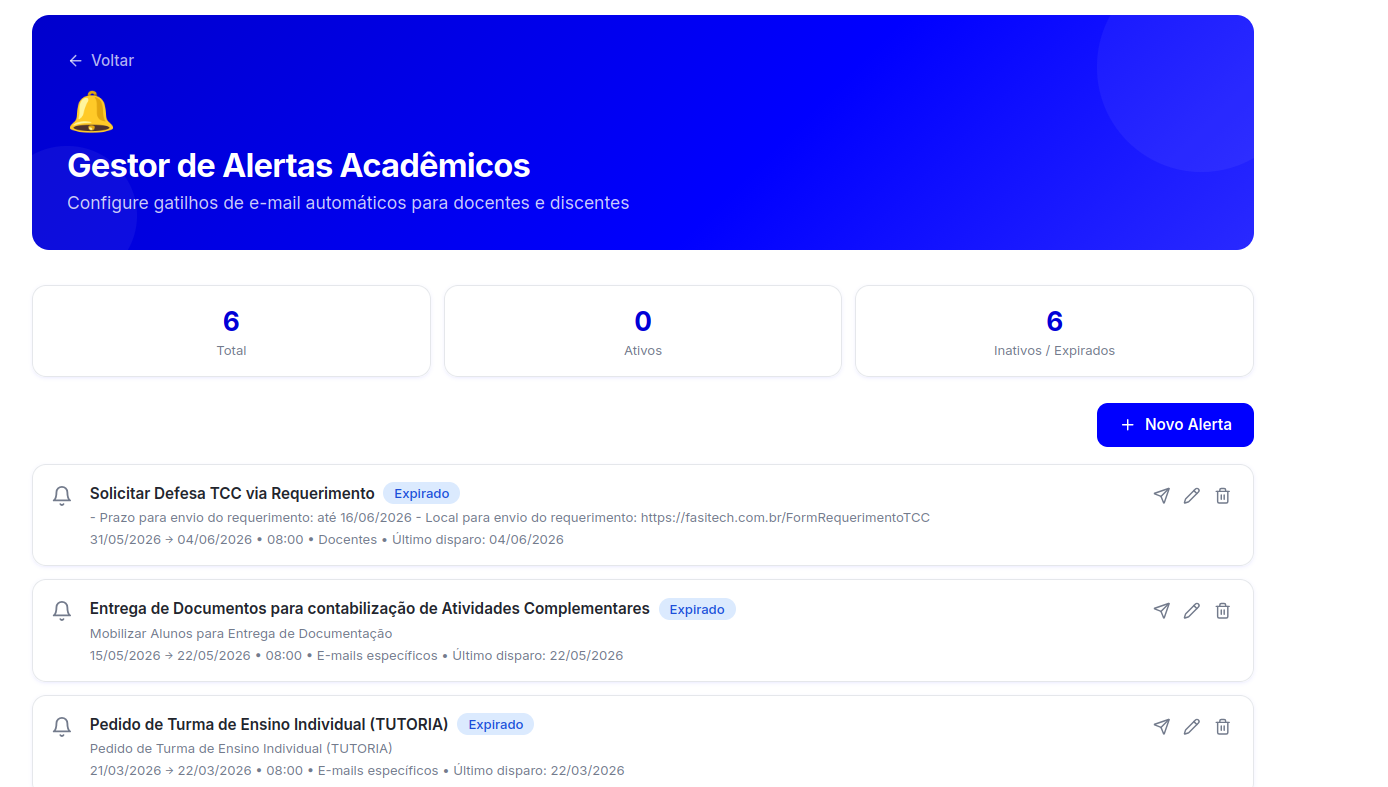
\includegraphics[width=0.49\linewidth]{GestorAlertas}\hfill%
  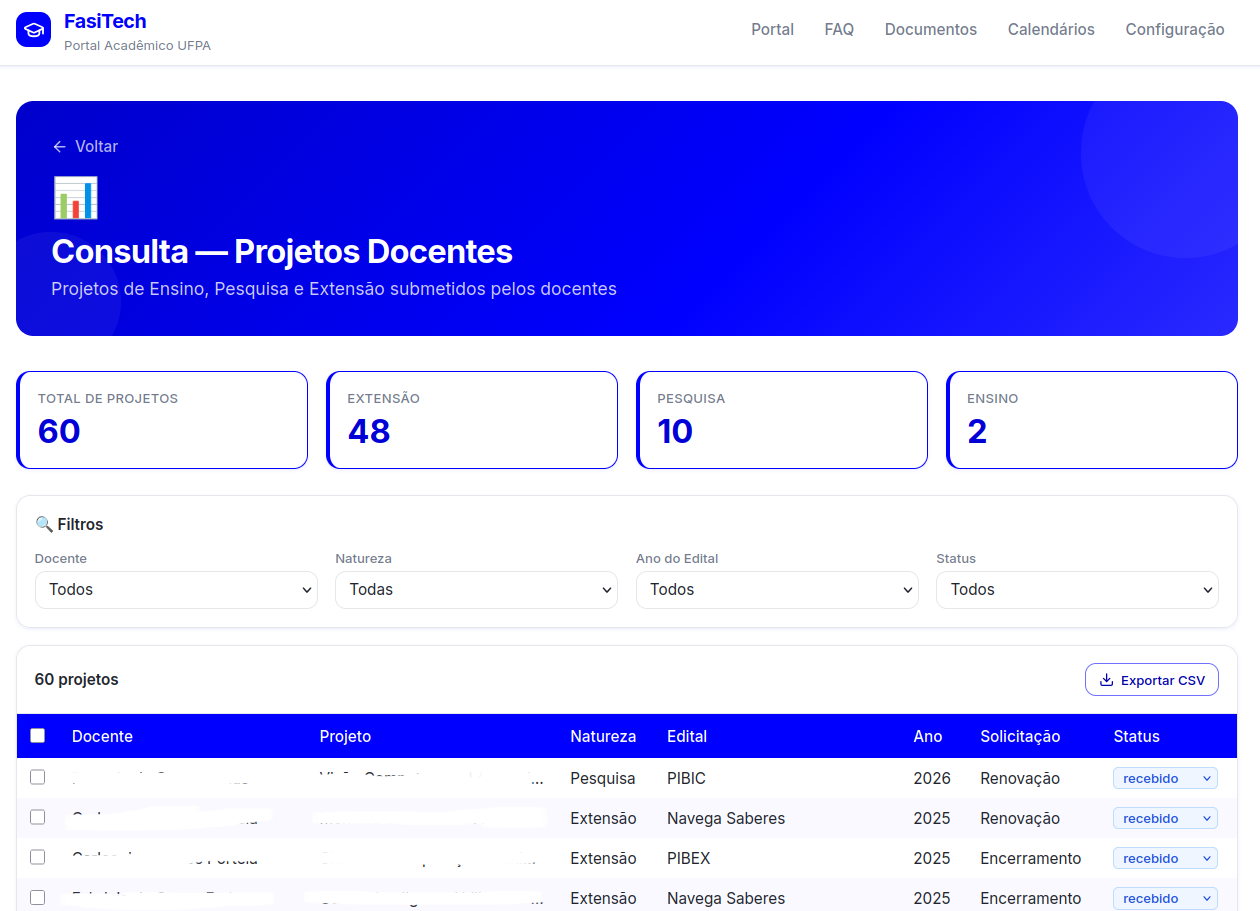
\includegraphics[width=0.49\linewidth]{ConsultaProjetos}\\[2pt]
  {\scriptsize\textit{Gestor de alertas: 6 disparos com 100\% de cumprimento de prazo (esq.).
  Consulta de 60 projetos docentes com filtros e exportação CSV (dir.).}}
\end{center}

\subsection*{7.2\;Impacto na equidade}

O resultado mais revelador é a distribuição geográfica: os dois polos \textit{mais
distantes} da sede administrativa concentram \textbf{75,7\% das submissões de ACC,
TCC e Estágio} $\rightarrow$ exatamente o grupo que mais sofria com o modelo presencial/papel
anterior. O FasiTech atende mais intensamente quem mais precisava de um canal remoto.

\begin{center}
\begin{tikzpicture}
\foreach \polo/\val/\col/\y in {
  {Polo Remoto A}/40.3/ufpablue!80/1.5,
  {Polo Remoto B}/35.4/ufpablue!55/0.75,
  {Polo Sede}/22.9/ufpablue!28/0.0
}{
  \fill[\col] (0,\y) rectangle (\val*0.12, \y+0.55);
  \node[left, font=\footnotesize, text width=3.5cm, align=right] at (-0.05, \y+0.27) {\polo};
  \node[right, font=\footnotesize\bfseries, text=ufpablue!80!black] at (\val*0.12+0.1, \y+0.27) {\val\%};
}
\draw[->] (0,-0.15) -- (5.2,-0.15);
\foreach \x/\lab in {1.2/10, 2.4/20, 3.6/30, 4.8/40} {
  \draw[gray!40] (\x,-0.1) -- (\x, 2.05);
  \node[below, font=\tiny, gray] at (\x,-0.15) {\lab\%};
}
\node[right, font=\tiny, gray] at (5.2,-0.15) {\% de envios};
\end{tikzpicture}
\end{center}

\subsection*{7.3\;Avaliação de satisfação (baseline)}

Avaliação de gestão (n\,=\,21, junho/2026): média geral \textbf{3,80\,/\,5,0};
\textbf{transparência = 4,05/5} (dimensão mais bem avaliada), planejamento = 3,89/5,
suporte = 3,84/5, comunicação = 3,84/5. A pergunta direta de impacto (Q12 --
\textit{``O FasiTech facilitou o envio e acompanhamento dos seus processos acadêmicos?''})
registrou \textbf{82\% de impacto positivo} (9 de 11 respostas válidas). As respostas abertas
apontam percepção positiva do canal digital e demandas por maior equidade no acesso
a oportunidades, insumo direto para planejamento da coordenação.

\begin{center}
  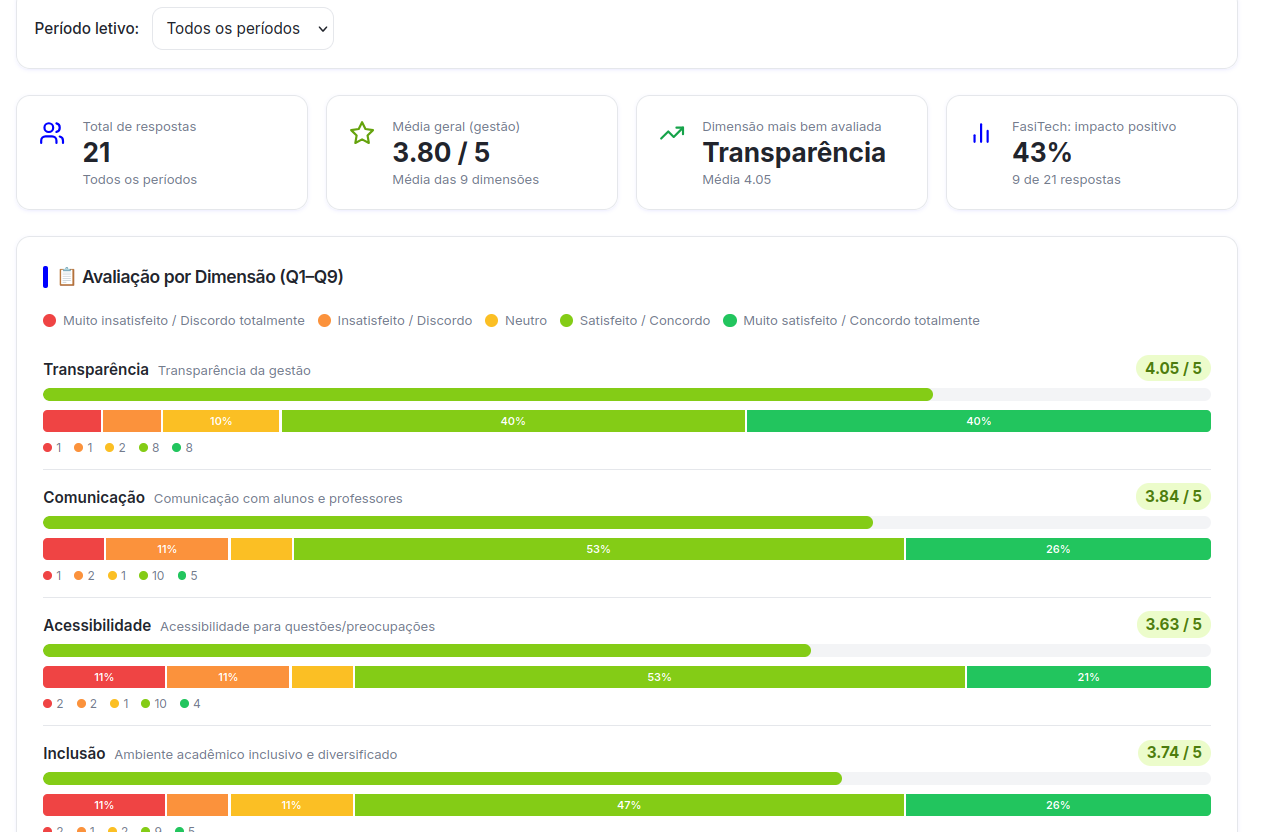
\includegraphics[width=0.90\linewidth]{DashboardGestao_View1}\\[4pt]
  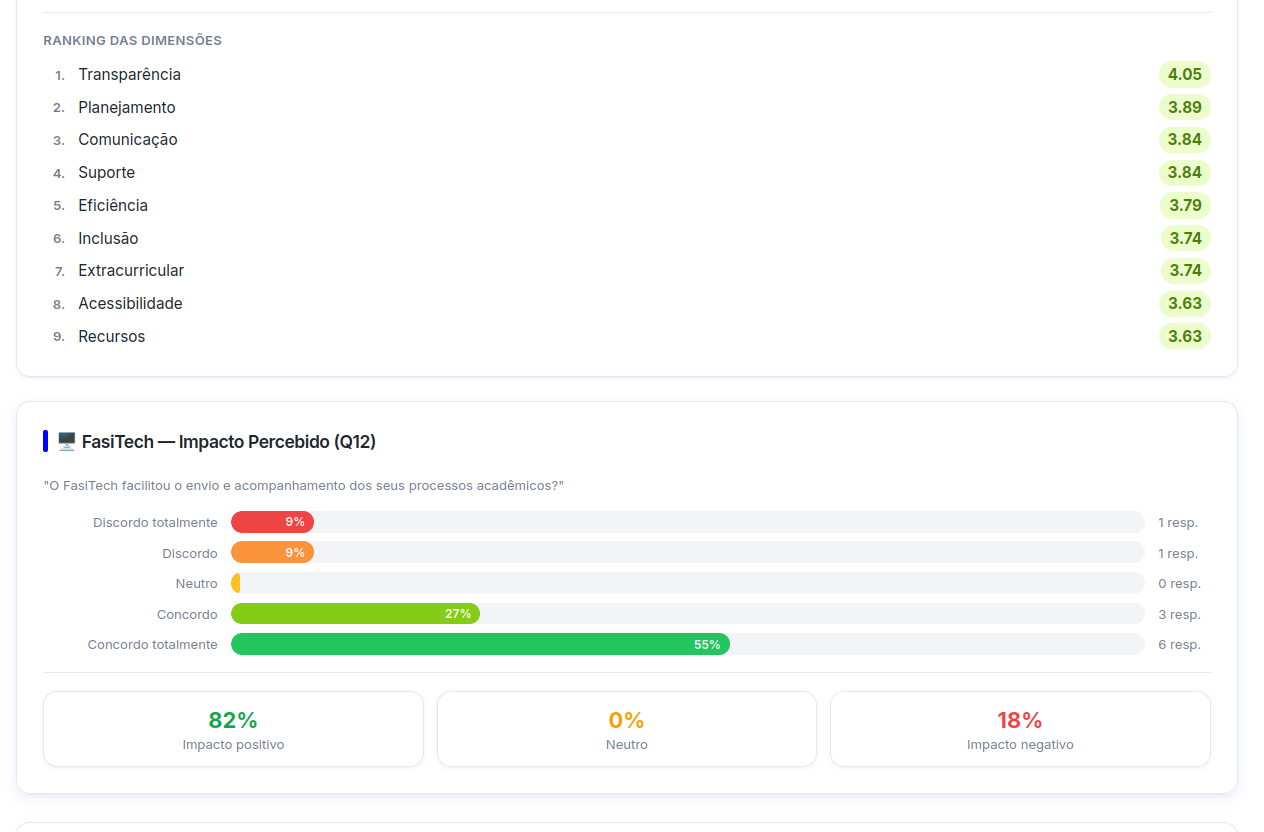
\includegraphics[width=0.90\linewidth]{DashboardGestaio_View2}\\[2pt]
  {\scriptsize\textit{Dashboard da Avaliação de Gestão: distribuição por dimensão (acima)
  e impacto percebido do FasiTech $\rightarrow$ 82\% positivo (abaixo).}}
\end{center}

% ============================================================
\section{8\;–\;Como os recursos foram utilizados?}
% ============================================================

\begin{center}
\renewcommand{\arraystretch}{1.2}
\begin{tabular}{L{2.8cm} L{4.5cm} L{5.5cm}}
\toprule
\textbf{Recurso} & \textbf{O que foi utilizado} & \textbf{Como foi otimizado} \\
\midrule
\textbf{Humano} &
  1 docente efetivo com expertise em desenvolvimento de sistemas &
  Desenvolvimento integrado às atividades de ensino e extensão; sem desvio de função nem custo adicional de pessoal \\
\addlinespace
\textbf{Tecnológico} &
  Servidor web de baixo custo; PostgreSQL (código aberto); API de IA (camada gratuita) &
  Evitou licenças proprietárias; stack 100\% open-source com suporte comunitário ativo \\
\addlinespace
\textbf{Financeiro} &
  Custo operacional $<$ R\$ 100,00/mês &
  Substituiu horas de secretaria em tarefas manuais; ROI imediato e positivo \\
\addlinespace
\textbf{Infraestrutura} &
  Laboratórios de informática e conectividade já disponíveis na unidade &
  Não exigiu aquisição de equipamentos adicionais \\
\bottomrule
\end{tabular}
\end{center}

\begin{tcolorbox}[warnbox]
  \textbf{\faLightbulb\;Eficiência mensurável:} O processo de análise manual de uma
  submissão de ACC consumia em média 15--20 minutos de secretaria. Com 53 submissões
  processadas por IA, estima-se uma economia de \textbf{mais de 13 horas-servidor} apenas
  neste módulo $\rightarrow$ sem contabilizar os ganhos dos outros 9 módulos digitalizados.
\end{tcolorbox}

% ============================================================
\section{9\;–\;Como a ação identificou as necessidades dos seus usuários/cidadãos?}
% ============================================================

O FasiTech foi concebido a partir de uma abordagem \textbf{centrada no usuário},
com múltiplos instrumentos de escuta ativa:

\begin{enumerate}[label={\color{ufpablue}\faBullseye}, leftmargin=2.2em, itemsep=4pt]
  \item \textbf{Observação direta dos processos de secretaria:} O mapeamento inicial
    partiu da observação do fluxo de trabalho cotidiano, identificando os gargalos de
    maior impacto (ACC manual, tramitação em papel, comunicação não rastreável).

  \item \textbf{Formulário socioeconômico como instrumento diagnóstico:} O módulo de
    dados socioeconômicos foi desenhado para capturar as variáveis que determinam a
    viabilidade do próprio sistema digital: conectividade, acesso a equipamentos,
    deslocamento, condição de trabalho e saúde mental.

  \item \textbf{Canal de voz qualitativo na Avaliação de Gestão:} O módulo inclui
    perguntas abertas que trouxeram demandas concretas não antecipadas, como a
    necessidade de protocolos de equidade em estágios de laboratório e maior
    transparência em processos de transferência de polo.

  \item \textbf{Dados de uso como retroalimentação contínua:} O sistema gera
    automaticamente métricas de uso (picos, módulos mais acessados, distribuição por
    polo) que informam prioridades de desenvolvimento e campanhas de comunicação.

  \item \textbf{Perguntas ao Diretor Virtual como mapeamento de lacunas:} As dúvidas
    mais frequentes ao assistente virtual revelam lacunas de informação nos materiais
    institucionais, sinalizando onde o PPC e os regulamentos precisam ser melhor
    comunicados.
\end{enumerate}

Esse ciclo de escuta, desenvolvimento e retorno está alinhado ao objetivo do PDI de
\textit{``aprimorar a comunicação institucional com linguagem clara e acessível, em
todos os suportes, plataformas e meios de comunicação disponíveis''}.

% ============================================================
\section{10\;–\;Quais são os mecanismos de transparência, publicidade e controle social que a ação promove?}
% ============================================================

\begin{itemize}[label={\color{ufpablue}\faLock}, itemsep=4pt]
  \item \textbf{Avaliação de Gestão com publicidade interna:} Estudantes e docentes
    avaliam a coordenação em 9 dimensões com escala 1--5 e campo aberto. Os resultados
    são consolidados e apresentados a coordenação, criando ciclo institucional de
    melhoria contínua. Resultado atual: \textbf{transparência = 4,43/5 $\rightarrow$ dimensão de
    maior pontuação na avaliação}.

  \item \textbf{Alertas acadêmicos com histórico auditável:} Cada notificação é
    armazenada com data de criação, data de disparo e público destinatário $\rightarrow$ histórico
    auditável de comunicações institucionais, com taxa de 100\% de cumprimento de prazo
    (6/6 alertas).

  \item \textbf{Rastreabilidade digital dos trâmites:} Cada submissão é registrada
    com data, polo de origem, módulo e identificação do usuário, permitindo à coordenação
    acompanhar o andamento dos processos e identificar gargalos de tramitação.

  \item \textbf{Dados socioeconômicos para políticas públicas internas:} Os 148 perfis
    estruturados, com mais de 20 variáveis, constituem a primeira base de dados sistemática
    para fundamentar solicitações ao PROAIS/UFPA e à assistência estudantil, tornando
    públicas, para a gestão, as condições reais de vida do corpo discente.

  \item \textbf{Acesso igualitário entre polos:} A plataforma elimina a assimetria
    informacional do modelo presencial: estudantes dos polos mais distantes
    têm o mesmo acesso a informações e processos que estudantes do polo sede.
\end{itemize}

% ============================================================
\section{11\;–\;Quais foram as principais barreiras encontradas no desenvolvimento da ação inovadora e como foram vencidas?}
% ============================================================

\begin{center}
\renewcommand{\arraystretch}{1.2}
\begin{tabular}{L{4.8cm} C{1.8cm} L{5.4cm}}
\toprule
\textbf{Barreira} & \textbf{Impacto} & \textbf{Como foi superada} \\
\midrule
Exclusão digital (14,2\% sem internet estável; 25\% sem computador próprio) &
  \textcolor{ufpared}{\textbf{Alto}} &
  Interface responsiva para smartphone; orientação para uso dos laboratórios da unidade \\
\addlinespace
Integração com SIGAA para automação plena de notas &
  \textcolor{ufpared}{\textbf{Alto}} &
  Módulo autônomo de lançamento de conceitos; integração com SIGAA definida como meta de próxima fase \\
\addlinespace
Adaptação de docentes e secretaria ao novo fluxo &
  \textcolor{accentor}{\textbf{Médio}} &
  Benefícios imediatos visíveis (menos trabalho manual); treinamento contextualizado e sem burocracia \\
\addlinespace
Zero orçamento adicional para desenvolvimento &
  \textcolor{accentor}{\textbf{Médio}} &
  Stack 100\% open-source; APIs de IA em camada gratuita; hospedagem de baixo custo \\
\addlinespace
Qualidade dos dados históricos (campos sem normalização) &
  \textcolor{accentor}{\textbf{Médio}} &
  Documentação das lacunas; correção incremental; campos obrigatórios nos novos formulários \\
\addlinespace
Desenvolvimento paralelo às obrigações docentes &
  \textcolor{accentor}{\textbf{Médio}} &
  Metodologia incremental por ciclos curtos; priorização por impacto imediato no usuário \\
\bottomrule
\end{tabular}
\end{center}

% ============================================================
\section{12\;–\;Quais foram os principais fatores que contribuíram para o sucesso da ação inovadora?}
% ============================================================

\begin{itemize}[label={\color{darkgreen}\faStar}, itemsep=5pt]
  \item \textbf{Orientação pela dor real:} O sistema nasceu da observação direta de
    problemas vividos cotidianamente pela comunidade acadêmica. Isso gerou aderência
    imediata: em outubro de 2025 (primeiro mês), 66 submissões foram realizadas sem
    nenhuma campanha de obrigatoriedade.

  \item \textbf{Perfil do executor na interseção técnica-acadêmica:} Um docente com
    competência em desenvolvimento de sistemas e vivência dos processos acadêmicos pôde
    traduzir necessidades institucionais em soluções digitais funcionais, sem
    intermediários que gerassem perda de requisitos ou atraso de entrega.

  \item \textbf{Desenvolvimento incremental e orientado a evidências:} Cada módulo
    foi lançado de forma independente, validado em uso real e ajustado antes de ampliar
    o escopo. O pico de 173 submissões em março/2026 confirma que o sistema
    entregou valor suficiente para gerar adesão espontânea.

  \item \textbf{Alinhamento explícito com o PDI da UFPA:} O FasiTech responde
    diretamente a objetivos do PDI 2016-2025, especialmente \textit{``melhorar e
    fortalecer a governança dos processos internos''}, \textit{``aprimorar a gestão
    acadêmica''} e \textit{``expandir a gestão na perspectiva multicampi''}. Esse
    alinhamento conferiu legitimidade institucional à iniciativa desde o início.

  \item \textbf{Sensibilidade ao contexto de vulnerabilidade:} O design da plataforma
    considerou desde o início as restrições reais do público (conectividade limitada,
    ausência de computador, necessidade de interface simples), resultando em uma
    ferramenta acessível na prática, não apenas no papel.

  \item \textbf{Instrumentalização da própria plataforma para gerar evidências:} A
    decisão de estruturar banco de dados com campos históricos e polo de origem desde o
    início permitiu extrair indicadores concretos de impacto $\rightarrow$ retroalimentando o
    desenvolvimento e fundamentando a expansão do sistema.
\end{itemize}

\begin{tcolorbox}[metricbox]
  \textbf{\faBullseye\;Síntese:} O sucesso do FasiTech demonstra que inovação
  organizacional efetiva no contexto universitário público resulta da combinação entre
  \textbf{vontade institucional} (legitimidade junto a coordenação e a comunidade),
  \textbf{competência técnica comprometida com o bem público} e \textbf{escuta ativa
  das necessidades dos usuários}. O sistema que os usuários \textit{efetivamente
  adotaram}, como os dados de uso comprovam, é a melhor evidência de que o
  problema certo foi resolvido da forma certa.
\end{tcolorbox}

% ============================================================
\section{13\;–\;Links de vídeos, áudios, imagens ou documentos}
% ============================================================

Os materiais de evidência da ação inovadora estão organizados nos seguintes artefatos,
disponíveis para verificação pela Comissão de Avaliação mediante solicitação:

\begin{itemize}[label={\color{ufpablue}\faLink}, itemsep=4pt]
  \item \textbf{Sistema em produção:} Plataforma web acessível pelos usuários
    cadastrados nos três polos -- em operação contínua desde outubro de 2025.

  \item \textbf{Relatório de Impacto (junho/2026):} Documento técnico com extração
    direta do banco de dados de produção contendo todos os indicadores quantitativos
    referenciados neste relato. Gerado automaticamente por consulta ao banco PostgreSQL
    em 03/06/2026.

  \item \textbf{Apresentação institucional com capturas de tela:} Documento PDF com
    imagens de todos os módulos em uso real, incluindo formulários de ACC, TCC, Estágio,
    Perfil Socioeconômico, Alertas Acadêmicos e interface do Diretor Virtual.

  \item \textbf{Repositório de código-fonte documentado:} Base tecnológica completa
    da plataforma, evidenciando a viabilidade de replicação em outros campi com
    custo e esforço mínimos.
\end{itemize}

\begin{center}
  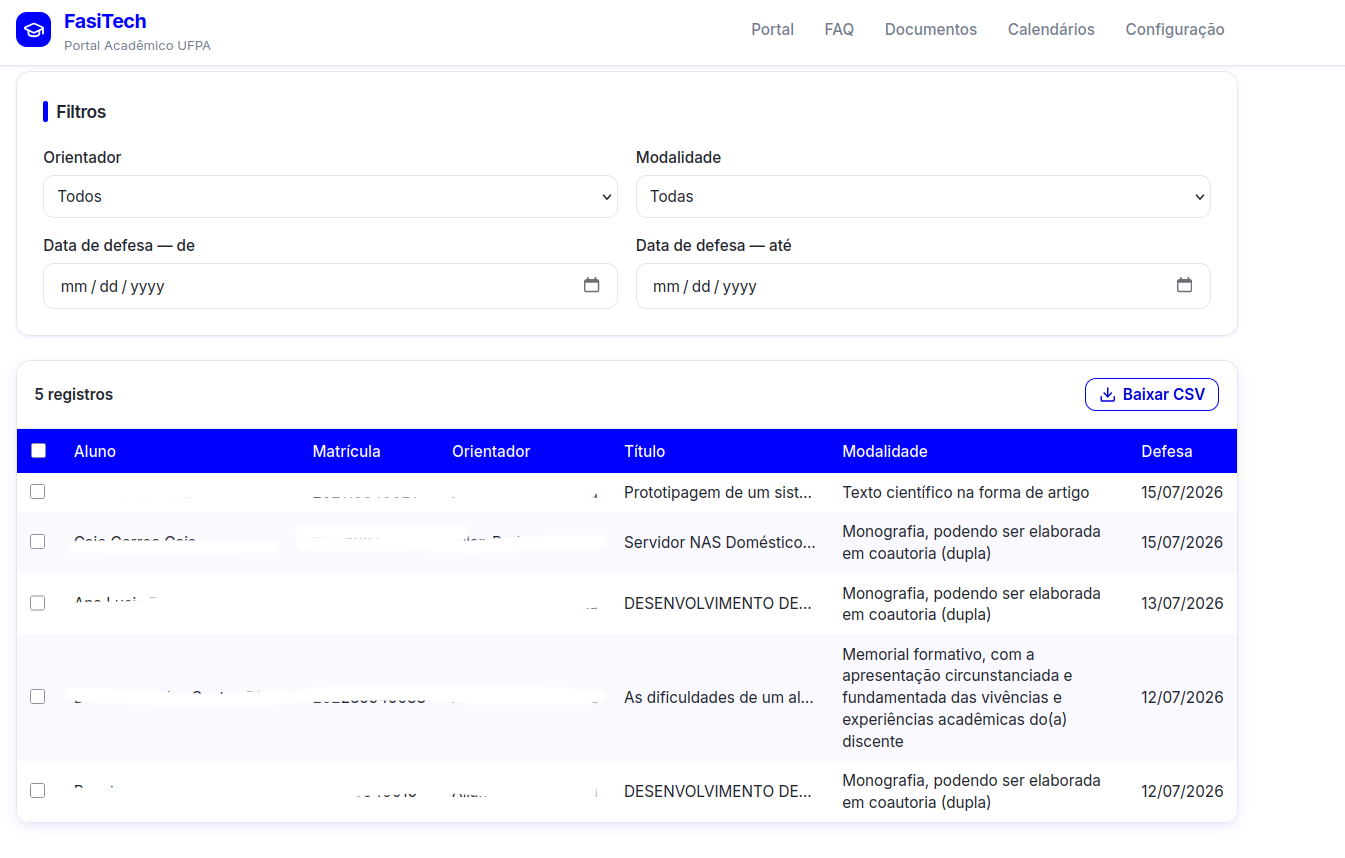
\includegraphics[width=0.75\linewidth]{ConsultaRequerimento}\\[2pt]
  {\scriptsize\textit{Consulta de requerimentos de banca TCC com filtros por orientador,
  modalidade e data de defesa -- exportação CSV disponível.}}
\end{center}

\begin{tcolorbox}[successbox]
  \textbf{\faClone\;Replicabilidade:} A arquitetura modular do FasiTech permite que
  qualquer subunidade multicampi da UFPA ative apenas os módulos pertinentes ao seu
  contexto. O custo estimado de implantação em nova unidade é inferior a 40 horas de
  configuração e treinamento, sem aquisição de licenças ou infraestrutura adicional.
  A experiência desta subunidade pode ser replicada em qualquer
  faculdade ou instituto com polos geograficamente dispersos, respondendo ao objetivo
  estratégico do PDI de \textit{``fomentar ações integradas entre os campi''}.
\end{tcolorbox}

\end{document}
